\chapter{THU THẬP THÔNG TIN VÀ TỔNG HỢP}
    \section{Các công trình có liên quan}
    \section{Tổng hợp kiến thức nền}
        \subsection{Cấu trúc cơ khí robot nhện}

        \hspace{0.5cm} Robot nhện 6 chân (hexapod) có cấu trúc cơ bản gồm một thân trung tâm (body) và 6 chân được bố trí đối xứng theo hai bên. Mỗi chân thường có 3 đoạn liên kết (link) kết nối qua 3 khớp quay:

        \begin{itemize}
            \item \textbf{Khớp Coxa:} Khớp gốc gắn vào thân, cho phép chân xoay trong mặt phẳng ngang (yaw). Đây là khớp xác định hướng của chân.
            \item \textbf{Khớp Femur:} Khớp giữa, cho phép chân nâng lên hoặc hạ xuống (pitch). Chiều dài đoạn femur ảnh hưởng trực tiếp đến tầm với của chân.
            \item \textbf{Khớp Tibia:} Khớp cuối, cho phép gấp/duỗi phần dưới chân (pitch). Cùng với femur, tibia quyết định độ cao và vị trí đầu chân.
        \end{itemize}

        Với 6 chân và 3 bậc tự do mỗi chân, robot có tổng cộng 18 bậc tự do chủ động (active DOF), đòi hỏi 18 servo hoạt động đồng thời. Cấu hình này cho phép mỗi chân định vị đầu chân (end-effector) tại bất kỳ điểm nào trong không gian làm việc của nó.

        \subsection{Động học robot (Kinematics)}

        \subsubsection{Động học thuận (Forward Kinematics)}

        \hspace{0.5cm} Động học thuận giải bài toán: \textit{Cho trước góc quay của các khớp, xác định vị trí và hướng của đầu chân trong không gian.}

        Đối với chân 3-DOF với các thông số hình học: chiều dài coxa $L_c$, femur $L_f$, tibia $L_t$, và các góc khớp $\theta_1$ (coxa), $\theta_2$ (femur), $\theta_3$ (tibia), vị trí đầu chân $(x, y, z)$ trong hệ tọa độ gắn với gốc khớp coxa được tính như sau:

        \begin{equation}
            p = L_c + L_f \cos\theta_2 + L_t \cos(\theta_2 + \theta_3)
        \end{equation}
        \begin{equation}
            x = p \cos\theta_1, \quad y = p \sin\theta_1
        \end{equation}
        \begin{equation}
            z = L_f \sin\theta_2 + L_t \sin(\theta_2 + \theta_3)
        \end{equation}

        trong đó $p$ là khoảng cách nằm ngang từ gốc coxa đến đầu chân.

        \subsubsection{Động học nghịch (Inverse Kinematics)}

        \hspace{0.5cm} Động học nghịch giải bài toán ngược: \textit{Cho trước vị trí đích $(x, y, z)$ của đầu chân, xác định các góc khớp $(\theta_1, \theta_2, \theta_3)$ cần thiết.}

        Đây là bài toán cốt lõi trong điều khiển robot nhện, vì người lập trình thường mô tả quỹ đạo chuyển động theo không gian Descartes (tọa độ $x, y, z$) thay vì trực tiếp theo góc servo.

        Với chân 3-DOF có hình học phẳng (femur và tibia nằm trong cùng một mặt phẳng), lời giải IK có thể tìm được bằng phương pháp hình học:

        \textbf{Bước 1:} Tính góc coxa từ hình chiếu xuống mặt phẳng ngang:
        \begin{equation}
            \theta_1 = \text{atan2}(y,\, x)
        \end{equation}

        \textbf{Bước 2:} Tính khoảng cách nằm ngang từ gốc femur đến đầu chân:
        \begin{equation}
            d = \sqrt{x^2 + y^2} - L_c
        \end{equation}

        \textbf{Bước 3:} Áp dụng định lý cosin cho tam giác femur--tibia--đầu chân:
        \begin{equation}
            \cos\theta_3 = \frac{d^2 + z^2 - L_f^2 - L_t^2}{2 L_f L_t}
        \end{equation}
        \begin{equation}
            \theta_3 = \text{atan2}\!\left(\pm\sqrt{1 - \cos^2\theta_3},\; \cos\theta_3\right)
        \end{equation}
        \begin{equation}
            \theta_2 = \text{atan2}(z,\, d) - \text{atan2}\!\left(L_t \sin\theta_3,\; L_f + L_t \cos\theta_3\right)
        \end{equation}

        Dấu $\pm$ trong $\theta_3$ tương ứng với hai cấu hình chân: \textit{elbow-up} và \textit{elbow-down}. Trong thực tế, robot nhện thường chọn cấu hình elbow-down để ổn định hơn.

        \subsection{Thuật toán dáng đi (Gait Algorithm)}

        \hspace{0.5cm} Dáng đi (gait) định nghĩa thứ tự và thời điểm nâng/đặt chân của robot trong một chu kỳ bước. Một gait được đặc trưng bởi:

        \begin{itemize}
            \item \textbf{Duty factor ($\beta$):} Tỉ lệ thời gian một chân tiếp đất trong một chu kỳ. $\beta > 0.5$ đảm bảo tính ổn định tĩnh.
            \item \textbf{Pha ($\phi_i$):} Độ lệch pha bắt đầu chu kỳ của chân thứ $i$ so với chân tham chiếu.
            \item \textbf{Swing phase:} Pha chân trên không, thực hiện quỹ đạo cung (arc trajectory) để bước tiến.
            \item \textbf{Stance phase:} Pha chân tiếp đất, đẩy thân robot về phía trước.
        \end{itemize}

        Các kiểu gait phổ biến với robot hexapod:

        \begin{table}[h!]
        \centering
        \caption{So sánh các kiểu dáng đi của robot hexapod}
        \label{tab:gait_compare}
        \begin{tabular}{|l|c|c|c|l|}
        \hline
        \textbf{Gait} & \textbf{Chân swing/lần} & \textbf{Duty factor} & \textbf{Tốc độ} & \textbf{Ổn định} \\
        \hline
        Tripod  & 3 & 0.5 & Cao   & Trung bình (3 điểm tựa) \\
        Ripple  & 2 & 0.67 & Trung bình & Cao (4 điểm tựa) \\
        Wave    & 1 & 0.83 & Thấp  & Rất cao (5 điểm tựa) \\
        \hline
        \end{tabular}
        \end{table}

        \textbf{Tripod gait} là lựa chọn phổ biến nhất trong các ứng dụng thực tế: 6 chân chia thành 2 nhóm tam giác (chân 1, 3, 5 và chân 2, 4, 6), hai nhóm xen kẽ nhau, đảm bảo robot luôn có 3 điểm tựa tạo thành tam giác bao quanh hình chiếu trọng tâm.

        \subsection{Điều khiển servo bằng PWM}

        \hspace{0.5cm} Servo RC (Radio Control) được điều khiển bằng tín hiệu PWM (Pulse Width Modulation) với chu kỳ 20 ms (tần số 50 Hz). Độ rộng xung điều khiển góc quay của servo:

        \begin{itemize}
            \item Xung 1000 µs $\rightarrow$ góc $0°$
            \item Xung 1500 µs $\rightarrow$ góc $90°$ (vị trí trung tính)
            \item Xung 2000 µs $\rightarrow$ góc $180°$
        \end{itemize}

        Trong thực tế, mối quan hệ giữa độ rộng xung $\tau$ (µs) và góc $\theta$ (độ) là tuyến tính:
        \begin{equation}
            \tau = \tau_{\min} + \frac{\theta}{180°} \cdot (\tau_{\max} - \tau_{\min})
        \end{equation}

        Với robot nhện sử dụng 18 servo, việc tạo 18 tín hiệu PWM độc lập vượt quá số lượng kênh phần cứng của hầu hết vi điều khiển thông dụng. Do đó, module mở rộng PCA9685 — một IC driver PWM 16 kênh giao tiếp qua I\textsuperscript{2}C — được sử dụng phổ biến để giải quyết vấn đề này. Có thể nối tiếp 2 module PCA9685 trên cùng một bus I\textsuperscript{2}C để đạt 32 kênh PWM độc lập.

        \subsection{Vi điều khiển và nền tảng nhúng}

        \hspace{0.5cm} Hệ thống điều khiển robot nhện yêu cầu một vi điều khiển có đủ năng lực xử lý để thực hiện đồng thời:

        \begin{itemize}
            \item Tính toán IK cho 6 chân theo thời gian thực.
            \item Quản lý giao tiếp I\textsuperscript{2}C với module PWM.
            \item Xử lý tín hiệu từ module điều khiển không dây.
            \item Thực thi vòng lặp điều khiển với tần số $\geq$ 50 Hz.
        \end{itemize}

        Các nền tảng vi điều khiển thường được sử dụng:

        \begin{table}[h!]
        \centering
        \caption{So sánh các nền tảng vi điều khiển}
        \label{tab:mcu_compare}
        \begin{tabular}{|l|c|c|c|}
        \hline
        \textbf{Nền tảng} & \textbf{Xung nhịp} & \textbf{RAM} & \textbf{Đặc điểm} \\
        \hline
        Arduino Mega 2560 & 16 MHz  & 8 KB   & Dễ lập trình, cộng đồng lớn \\
        STM32F103         & 72 MHz  & 20 KB  & Hiệu năng cao, giá rẻ \\
        ESP32             & 240 MHz & 520 KB & Tích hợp WiFi/Bluetooth \\
        Raspberry Pi Zero & 1 GHz   & 512 MB & Linux, xử lý ảnh được \\
        \hline
        \end{tabular}
        \end{table}

        Với yêu cầu của đề tài, STM32 hoặc ESP32 là lựa chọn phù hợp: đủ tốc độ xử lý cho thuật toán IK, hỗ trợ I\textsuperscript{2}C phần cứng cho PCA9685, và có thể tích hợp giao tiếp không dây.

        \subsection{Giao tiếp không dây}

        \hspace{0.5cm} Điều khiển robot từ xa có thể được thực hiện qua nhiều giao thức không dây. Trong phạm vi đề tài, hai lựa chọn chính được xem xét:

        \textbf{Bluetooth (HC-05 / HC-06):} Phạm vi khoảng 10 m, giao tiếp UART đơn giản, không cần cơ sở hạ tầng mạng, độ trễ thấp ($<$ 20 ms). Phù hợp cho điều khiển tay cầm hoặc ứng dụng điện thoại.

        \textbf{WiFi (ESP8266 / ESP32):} Phạm vi rộng hơn, hỗ trợ giao thức TCP/UDP, cho phép điều khiển qua trình duyệt web hoặc ứng dụng mạng. ESP32 tích hợp cả WiFi và Bluetooth trên cùng một chip, là lựa chọn linh hoạt cho các dự án robot.
   
    \section{Các sản phẩm tham khảo}

        \hspace{0.5cm} Trong quá trình nghiên cứu và định hướng thiết kế, nhóm đã khảo sát một số mô hình robot chân tiêu biểu trên thế giới để làm cơ sở so sánh và lựa chọn phương án phù hợp.

        \subsection{Robot MiniRHex}
            \begin{figure}[H]
                \centering
                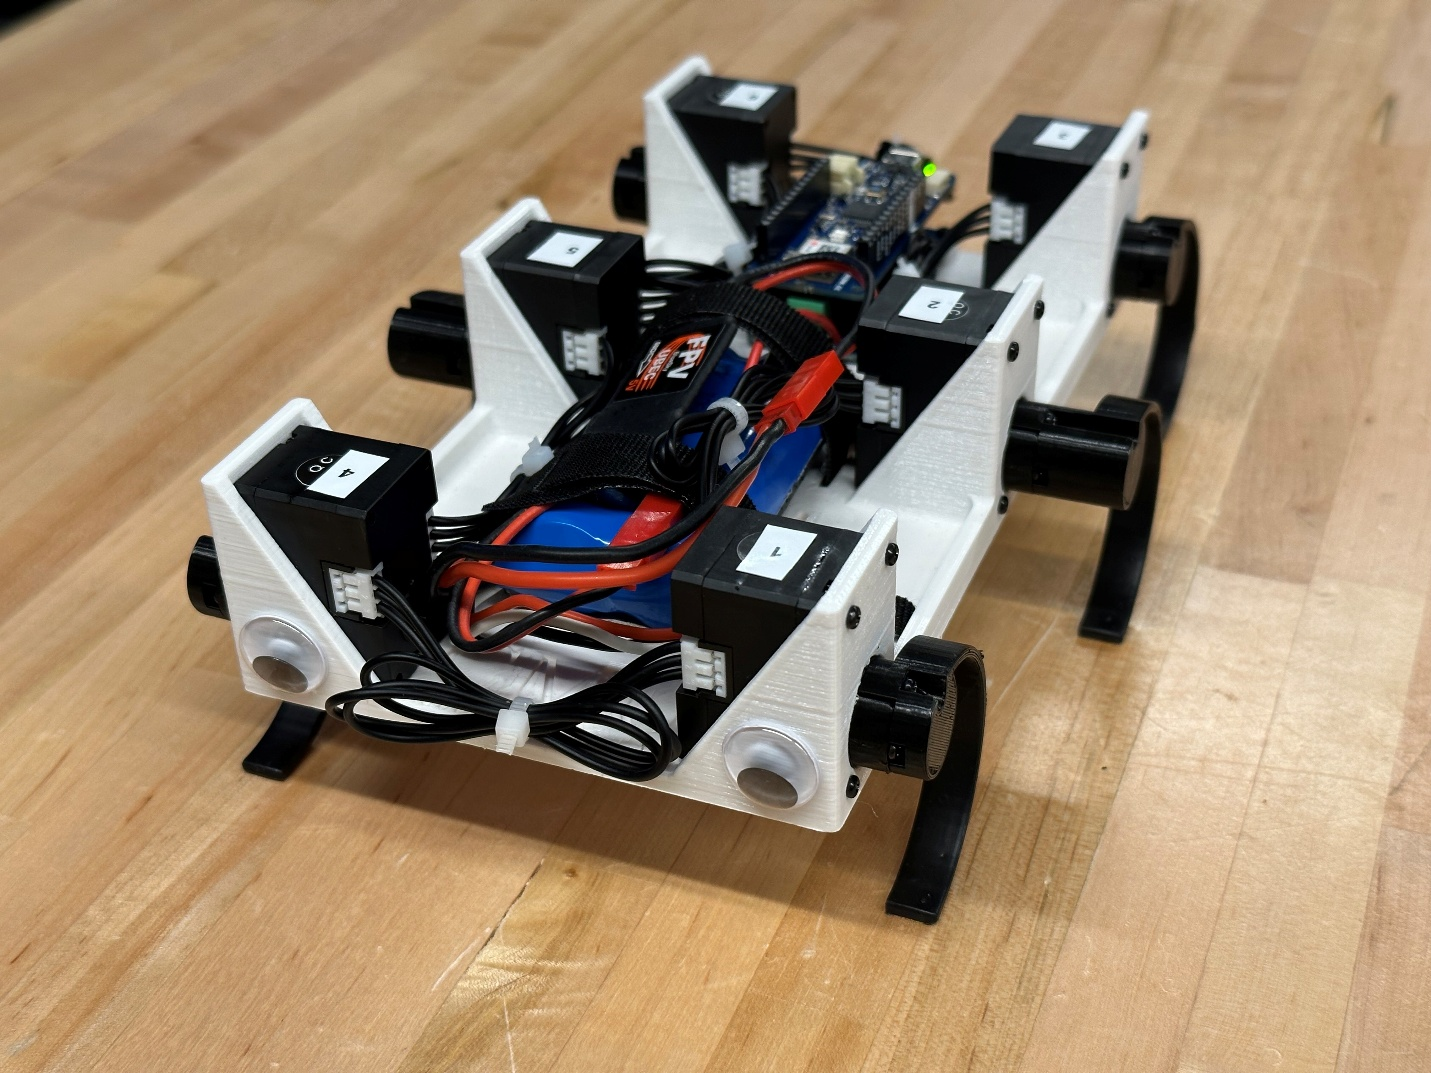
\includegraphics[width=0.75\textwidth]{pictures/minirhex.png}
                \caption{Robot MiniRHex}
            \end{figure}

            \hspace{0.5cm} MiniRHex là một phiên bản robot 6 chân nhỏ gọn lấy cảm hứng từ thiết kế RHex. Điểm đặc trưng của robot này là sử dụng chân đàn hồi hình chữ C, mỗi chân chỉ cần một động cơ điều khiển, giúp đơn giản hóa đáng kể cơ cấu truyền động so với các thiết kế chân đa khớp.

            \hspace{0.5cm} Thành phần phần cứng chính:
            \begin{itemize}
                \item Vi điều khiển trung tâm \textbf{ESP32}.
                \item 6 động cơ -- mỗi chân chỉ cần 1 động cơ quay liên tục.
                \item Chân đàn hồi hình chữ C được chế tạo từ vật liệu có tính đàn hồi cao.
                \item Cảm biến IMU (BNO055 hoặc MPU6050) để xác định góc nghiêng và gia tốc thân robot trong không gian.
                \item 6 mạch cầu H độc lập để điều khiển tốc độ và đảo chiều 6 động cơ.
            \end{itemize}

            \begin{figure}[H]
            \centering
            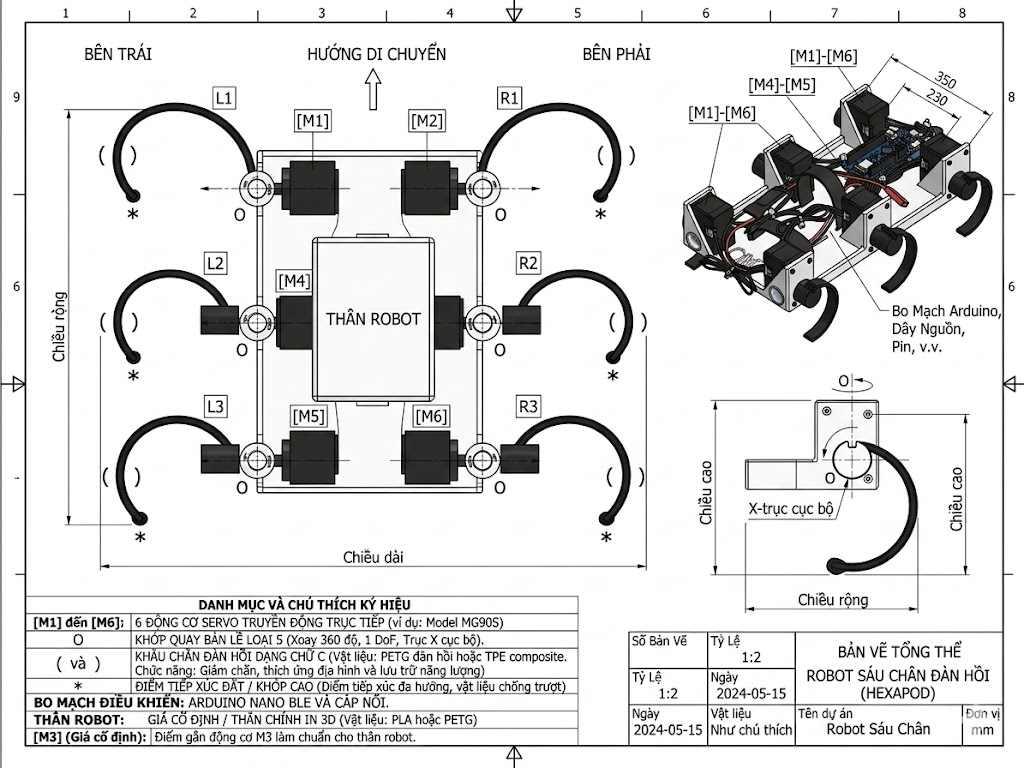
\includegraphics[width=0.75\textwidth]{pictures/minirhex_mechanical.png}
            \caption{Sơ đồ nguyên lý máy của MiniRHex}
            \end{figure}
            
            \begin{figure}[H]
            \centering
            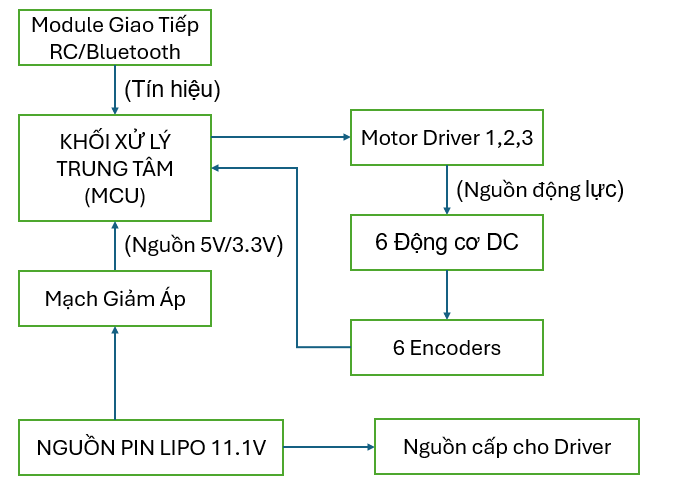
\includegraphics[width=0.75\textwidth]{pictures/minirhex_electrical.png}
            \caption{Sơ đồ khối hệ thống điện MiniRHex}
            \end{figure}

            \begin{figure}[H]
            \centering
            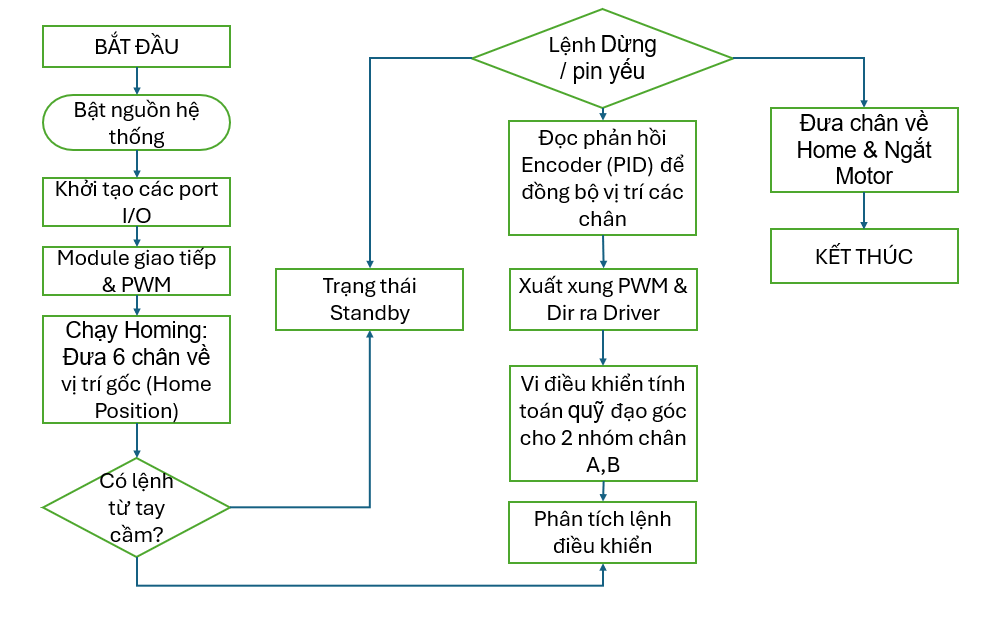
\includegraphics[width=0.75\textwidth]{pictures/minirhex_flowchart.png}
            \caption{Lưu đồ quy trình vận hành MiniRHex}
            \end{figure}

        \subsection{Robot miniHexa (Hiwonder)}

            \hspace{0.5cm} miniHexa là robot hexapod thương mại của hãng Hiwonder, hướng đến ứng dụng giáo dục và nghiên cứu. Robot tích hợp nhiều cảm biến và module AI, cho phép lập trình các tác vụ nhận dạng thị giác và phản hồi giọng nói.
            \begin{figure}[H]
                \centering
                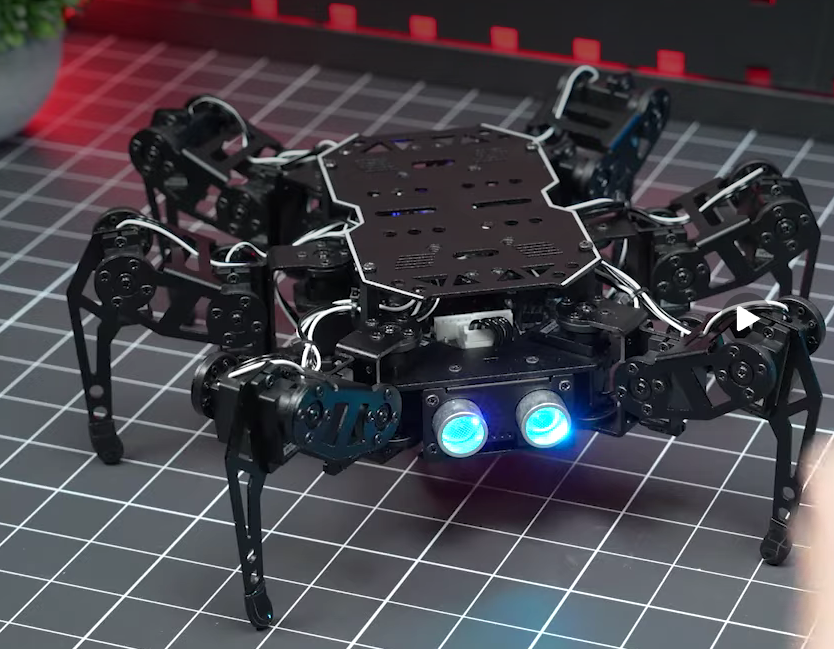
\includegraphics[width=0.75\textwidth]{pictures/minihexa.png}
                \caption{Robot miniHexa của Hiwonder}
            \end{figure}
            \hspace{0.5cm} Thành phần phần cứng chính:
            \begin{itemize}
                \item Vi điều khiển trung tâm \textbf{ESP32}.
                \item 18 micro servo tốc độ cao có tính năng chống kẹt.
                \item Module AI Vision để xử lý thị giác máy tính.
                \item Module nhận diện và phát giọng nói.
                \item Cảm biến siêu âm (phát sáng RGB), cảm biến chạm và cảm biến góc nghiêng IMU.
            \end{itemize}

            \begin{figure}[H]
            \centering
            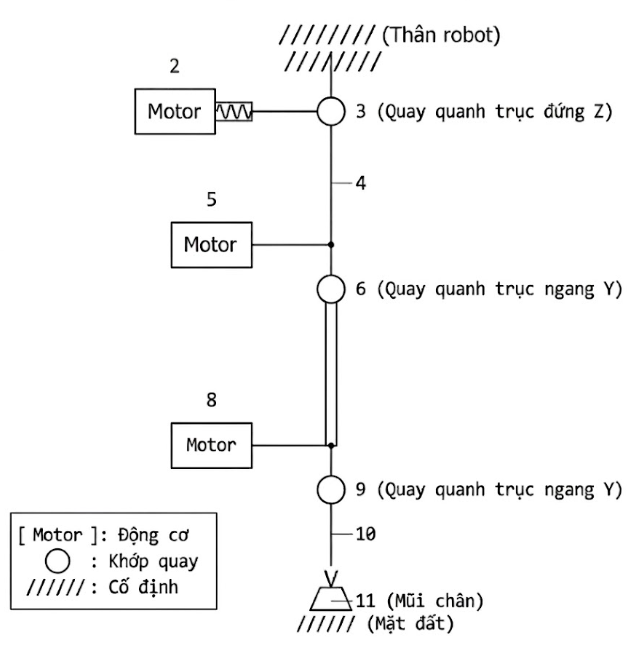
\includegraphics[width=0.75\textwidth]{pictures/hiwonder_mechanical.png}
            \caption{Sơ đồ nguyên lý máy của Hiwonder}
            \end{figure}

            \begin{figure}[H]
            \centering
            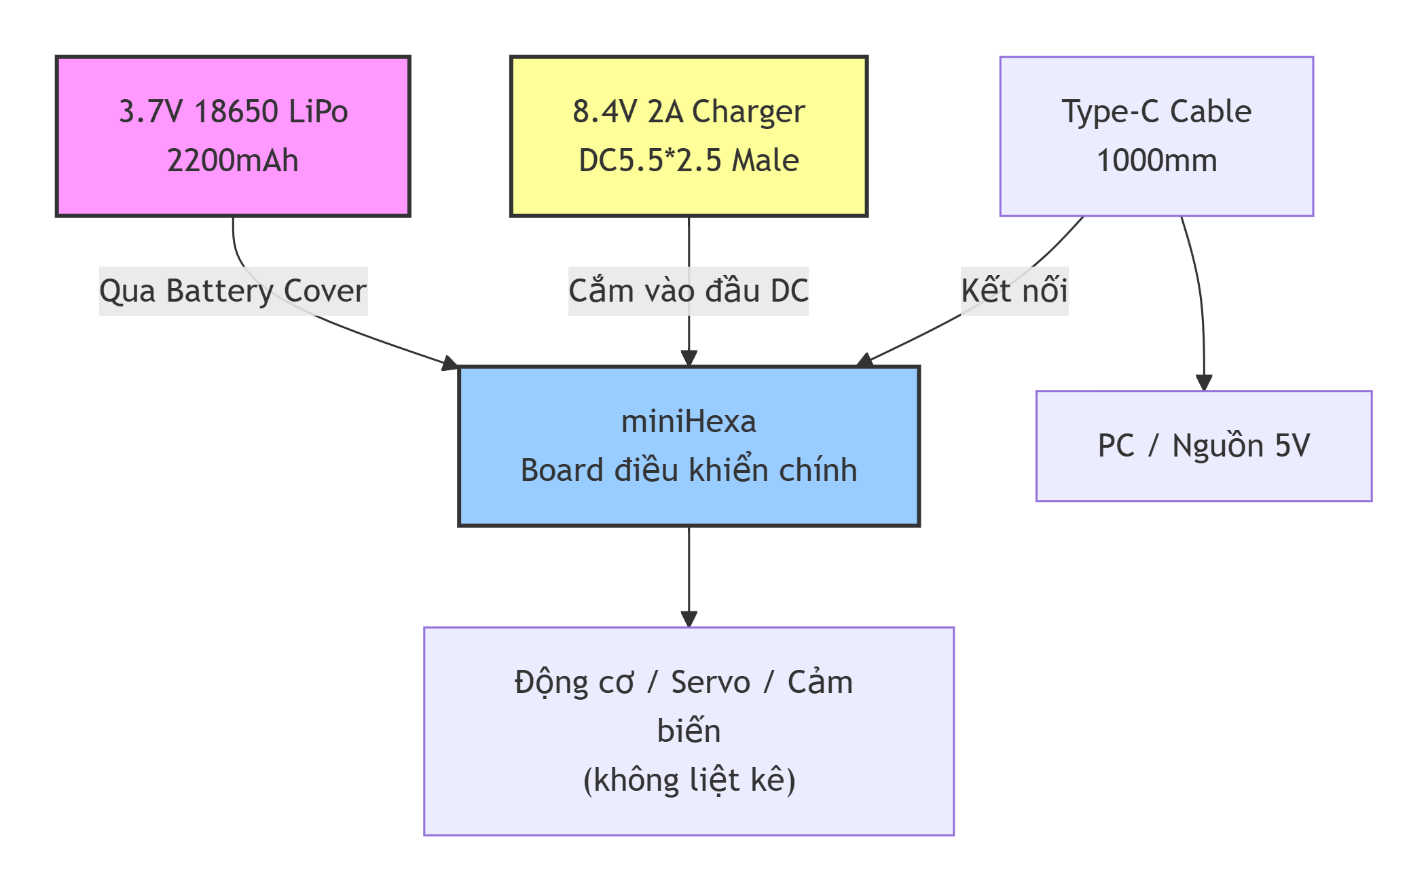
\includegraphics[width=0.75\textwidth]{pictures/hiwonder_electrical.png}
            \caption{Sơ đồ khối điện của Hiwonder}
            \end{figure}

            \begin{figure}[H]
            \centering
            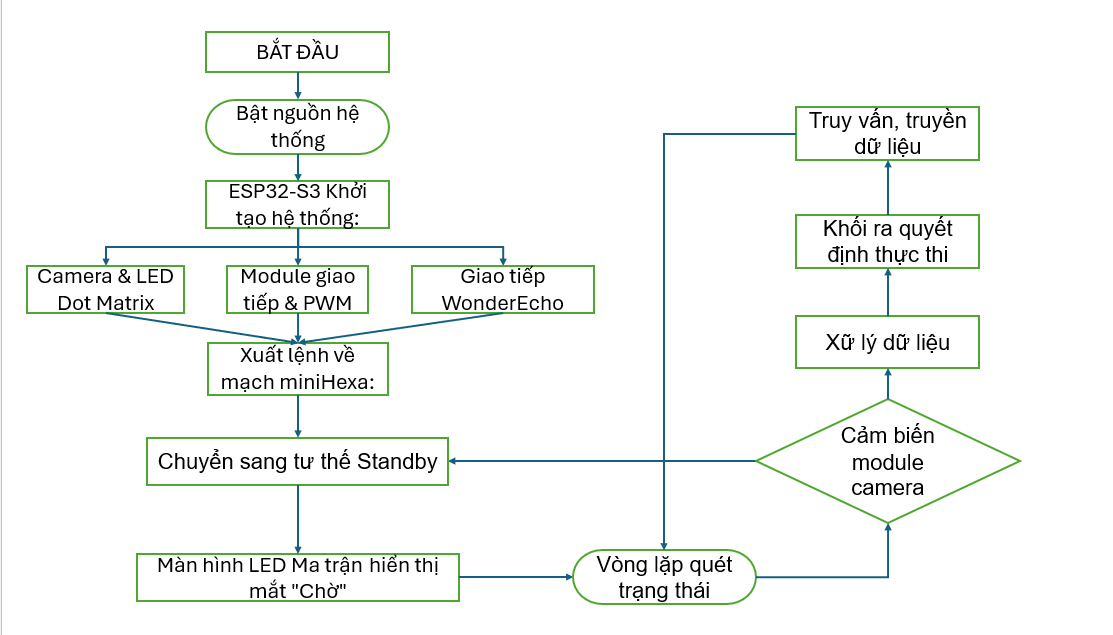
\includegraphics[width=0.75\textwidth]{pictures/hiwonder_flowchart.png}
            \caption{Lưu đồ quy trình vận hành Hiwonder}
            \end{figure}

       
